%!TEX root = ../report.tex
%*******************************************************************************
%                           Requirements Analysis                              %
%*******************************************************************************


\chapter{Requirements Analysis}

%******************************** Section 3.1 *********************************%
\section{Introduction}
    This chapter is about the overall vue of the project analysis and requirements.
    We start with analysing the global system and explaining its basic architecture then we illustrate that with a general
    sequence diagrams. In a second section we specify the project requirements and give a brief explanation of each one of
    them.

%******************************** Section 3.2 *********************************%
\section{Global System Analysis}

    \subsection{iExec ecosystem}
        iExec creates a global and open market where computing power is traded like a commodity. Its uses the blockchain
        as the laying underground so everything is certified on top of it. This guarantees multiple services such as
        the payments and the PoCo (...).
        This plateform has different agents\cite{iexec-architecture}:
        \begin{itemize}
            \item \textbf{The user} who issues computing resources to run decentralized applications. He is identified by
            his wallet and uses RLC to pay for the rented resources.

            \item \textbf{The worker} or resource provider who lends his machine power and monetize it. The worker builds his
            reputation according to executions he does.
            
            \item \textbf{The scheduler} manages the match-making of the demand and supply in the marketplace, does the
            necessary controls during the different phases of the process and finalizes the payments as well as sending
            results back to users.

            \item \textbf{The application developer} designs applications running on the Ethereum\cite{ethereum} blockchain.
        \end{itemize}

        \begin{landscape}
            \begin{figure}
                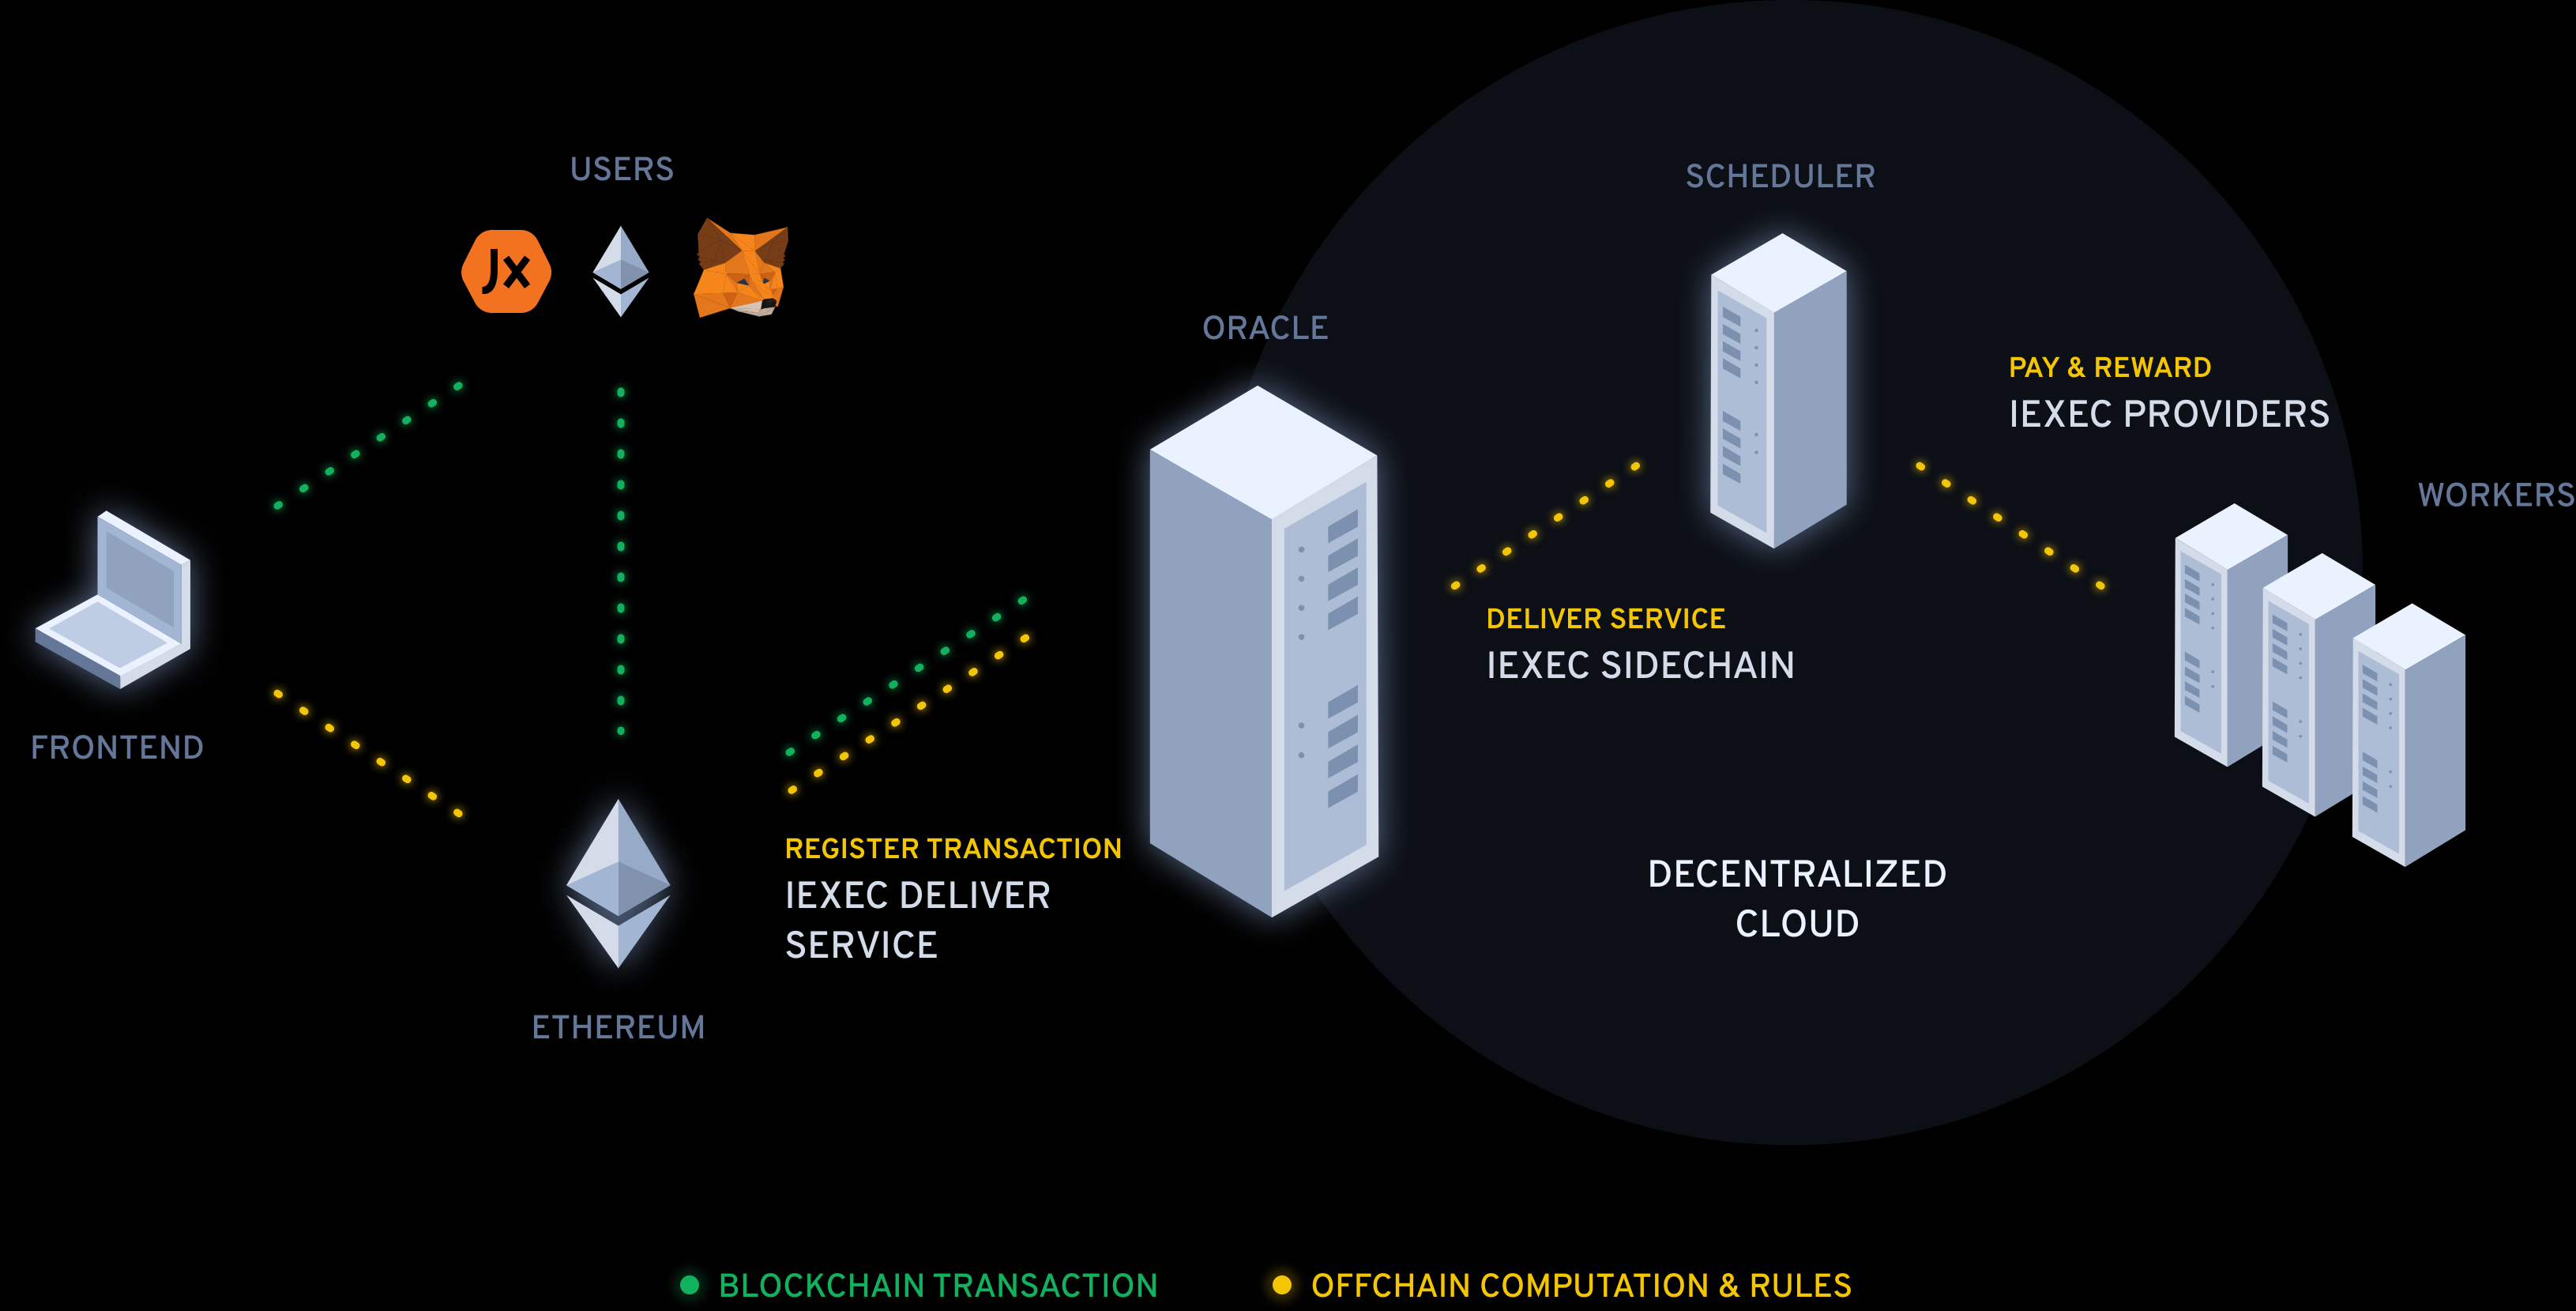
\includegraphics[width=\columnwidth]{4-Requirements/figs/iexec-decentralized-cloud.png}
                \caption{iExec decentralized cloud architecture}
            \end{figure}
        \end{landscape}

        The following figure\cite{iexec-marketplace} presents the iExec ecosystem and highlights the different parts of it
        including the marketplace and the worker pools.

        \begin{figure}[!h]
            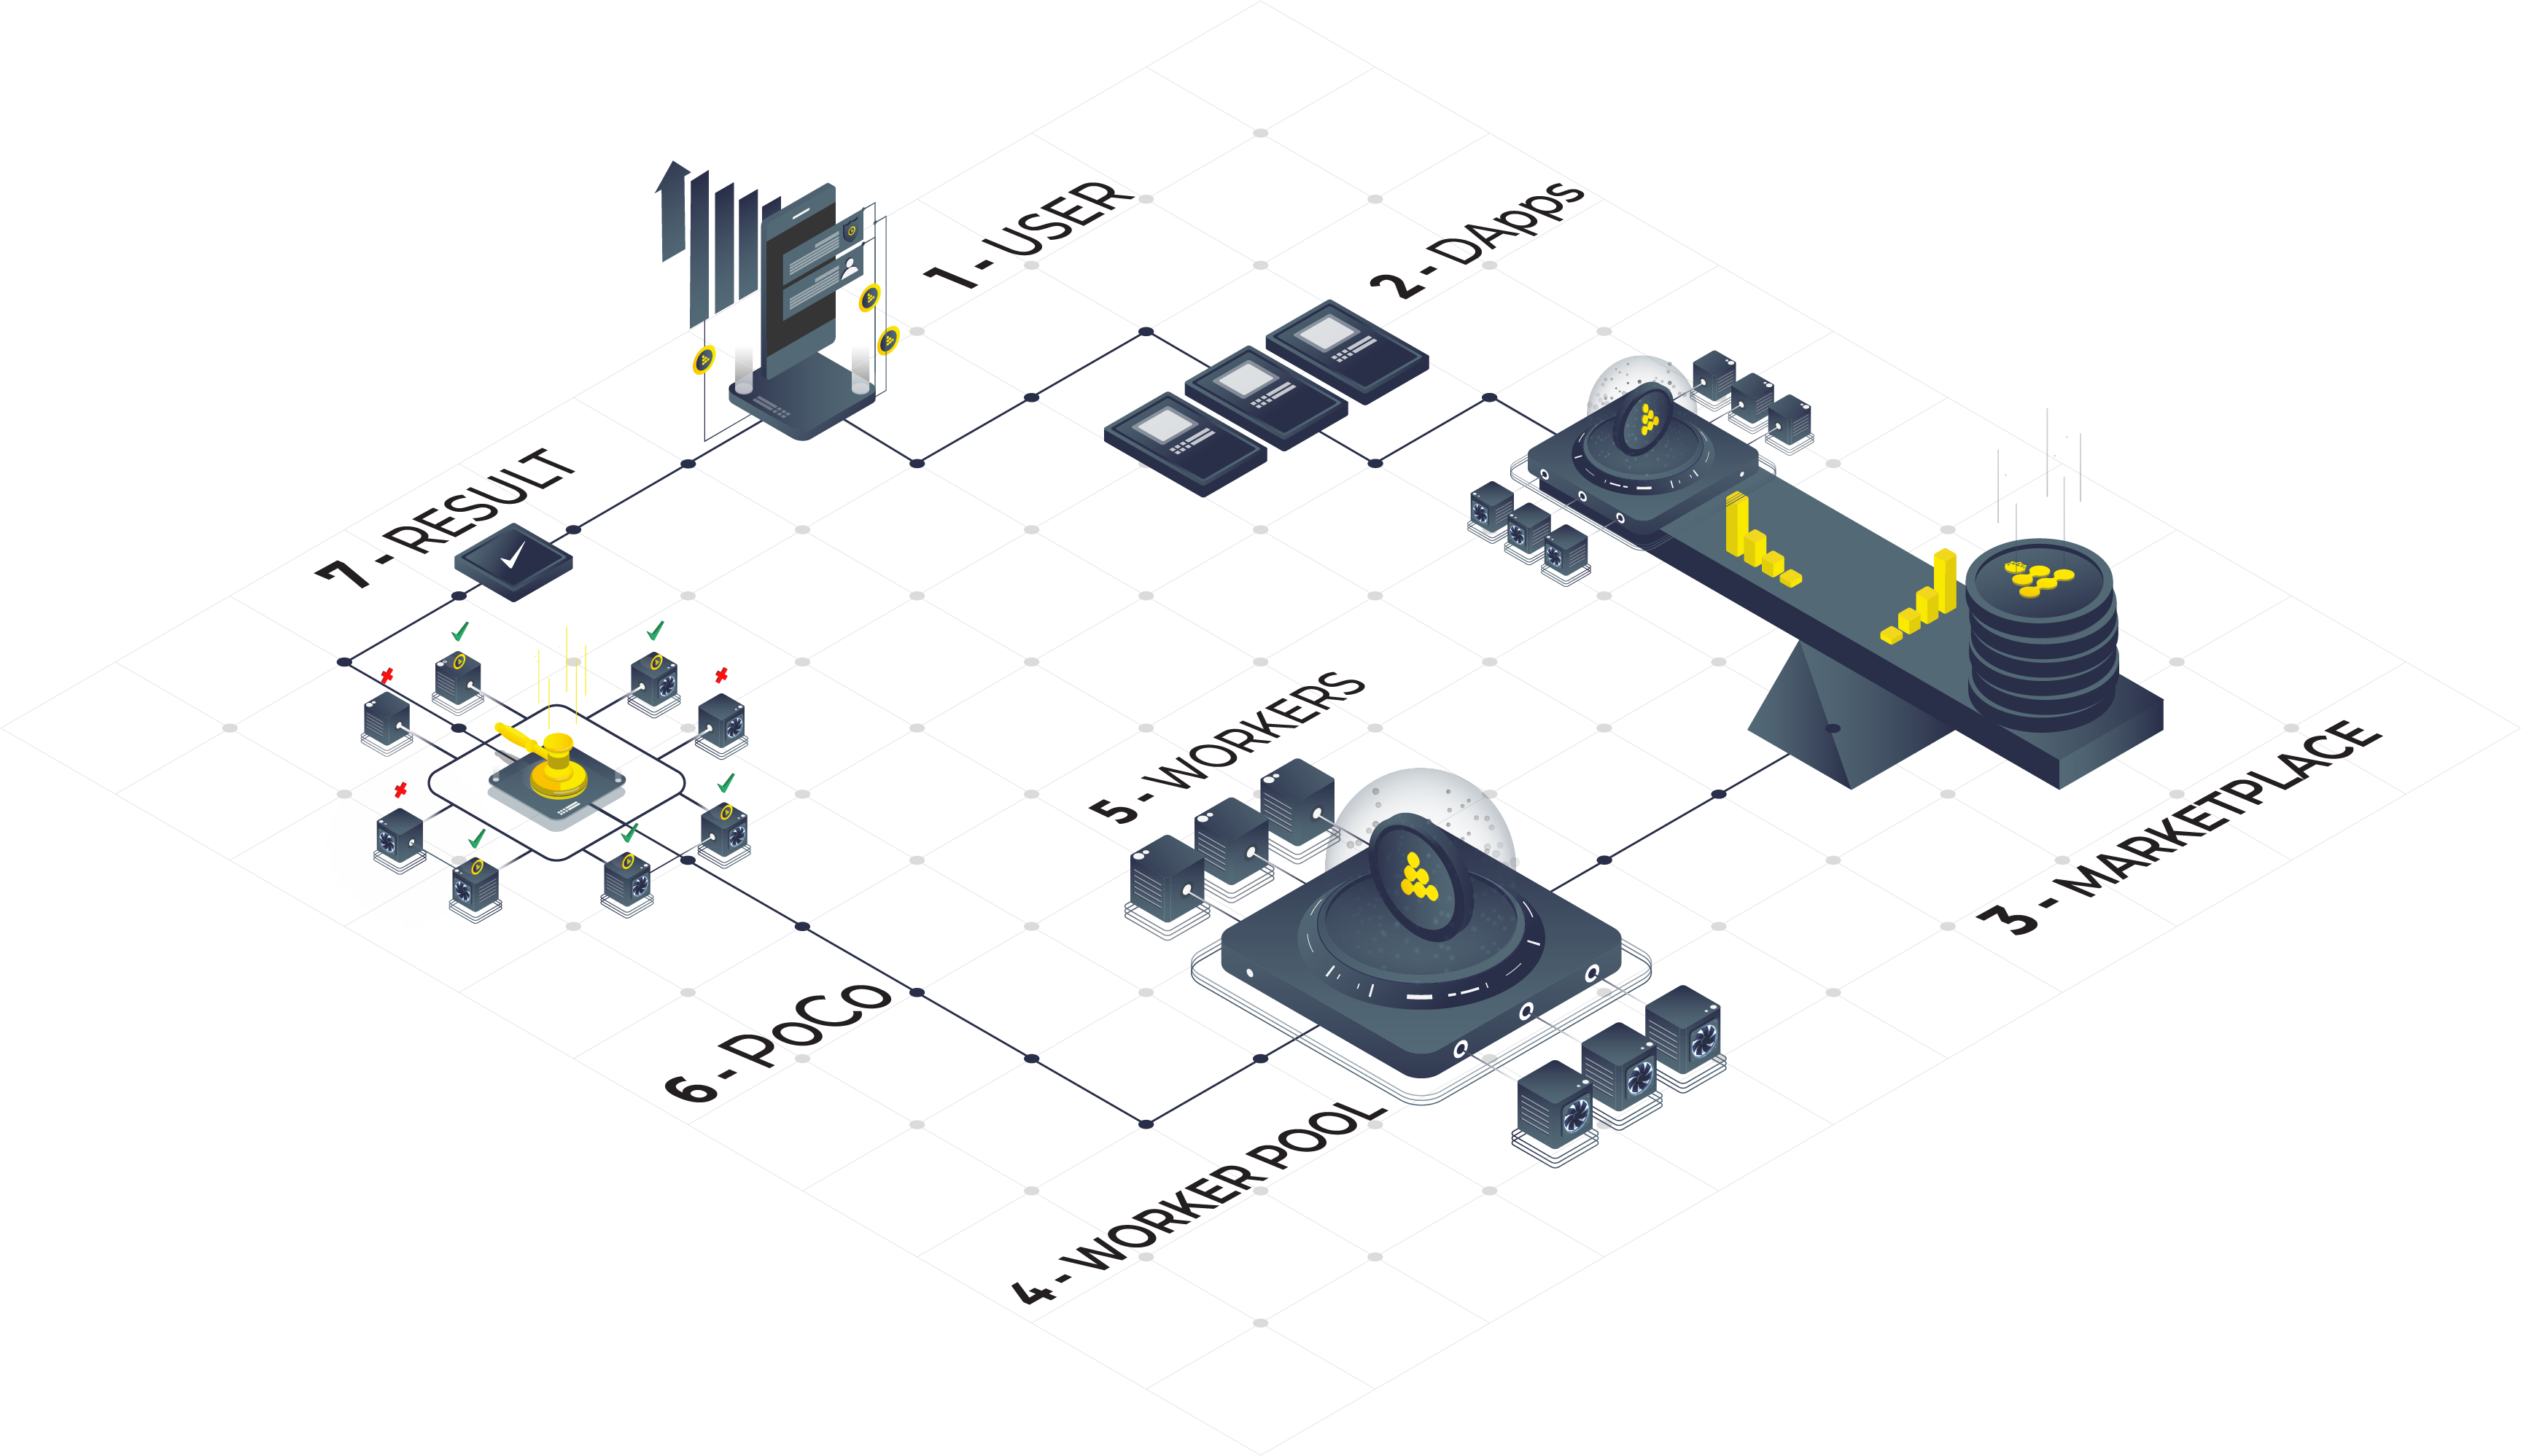
\includegraphics[width=\columnwidth]{4-Requirements/figs/iexec-marketplace.png}
            \caption{iExec marketplace}
        \end{figure}

    \subsection{General Sequence Diagram}
        The worker is one of three components of the global architecture, in addition to the scheduler and the user.
        The user starts the process by issuing and order (sending a job to be executed). The scheduler does the verification
        of the funds for all parts. It checks the accounts of the user and the worker and insures that they have enough RLC,
        delegates the job to the worker, gets the result, runs the PoCo to verify the execution, if no problem occurs it
        finalizes the payment and sends the result back to the user. The worker's mission starts once the job is delegated,
        it downloads the docker image of the application, downloads also the data needed by the execution, executes the task
        and uploads the result back to the scheduler. The worker has always to communicate with the scheduler to update his
        status (alive, working, waiting for work...) and give the scheduler the ability to track the execution process.\newline

        The sequence diagram illustrates the details of all the process:
        
        \begin{figure}[p]
            \vspace*{-2cm}
            \makebox[\linewidth]{
                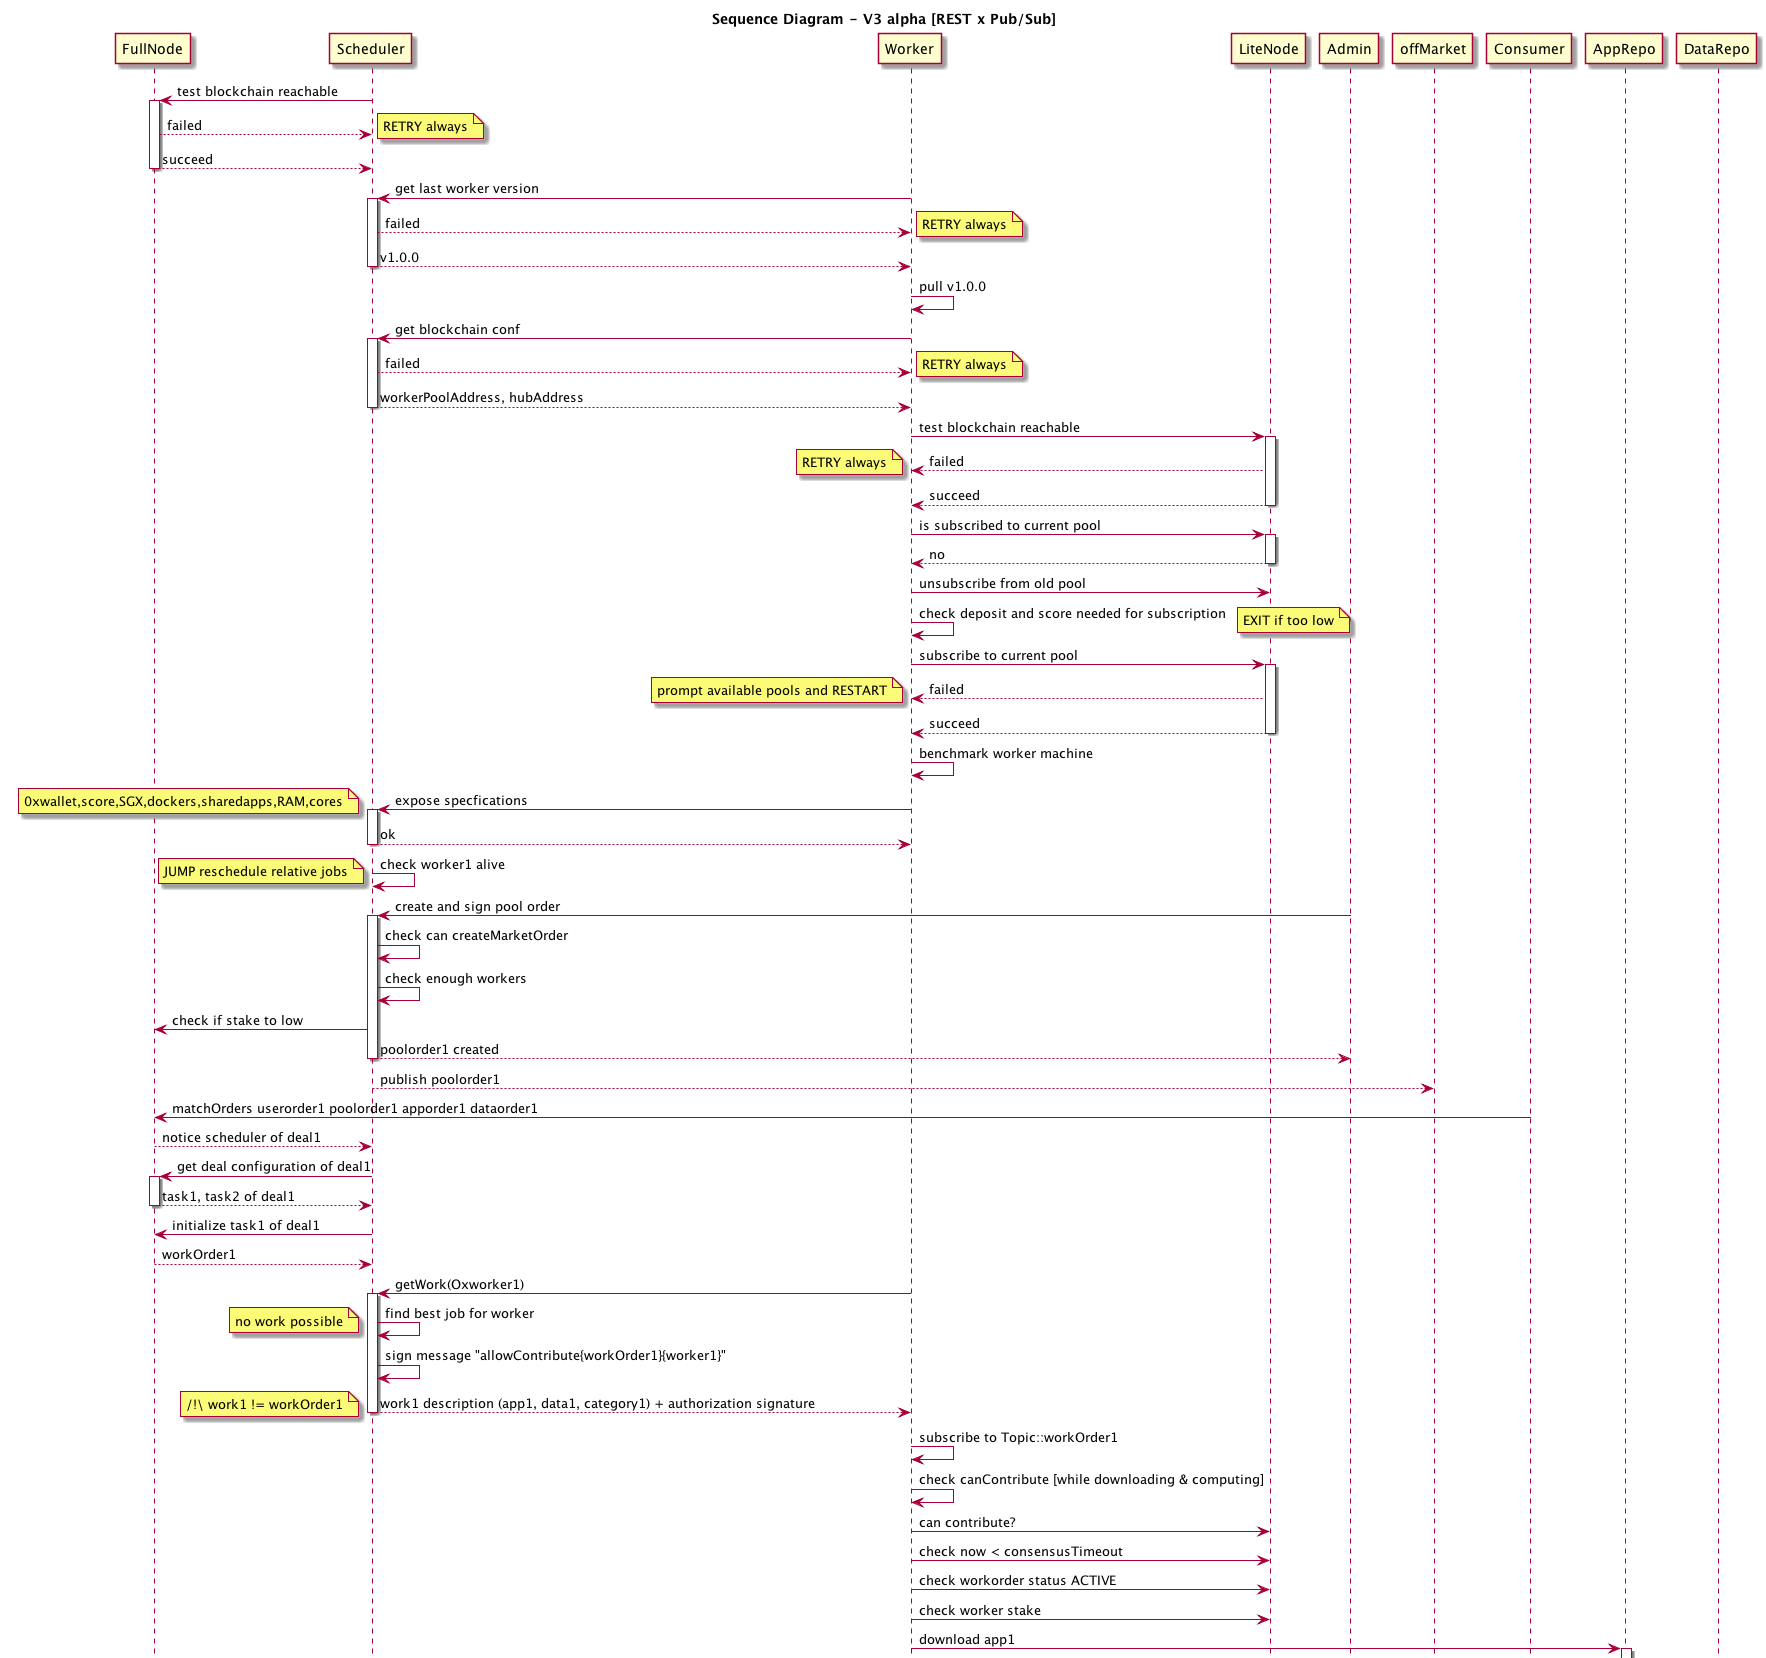
\includegraphics[width=1.3\linewidth]{4-Requirements/figs/iexec-core-sequence-diagram-part-1.png}
            }
            \caption{iExec core sequence diagram - part 1}
        \end{figure}

        \begin{figure}[p]
            \vspace*{-2cm}
            \makebox[\linewidth]{
                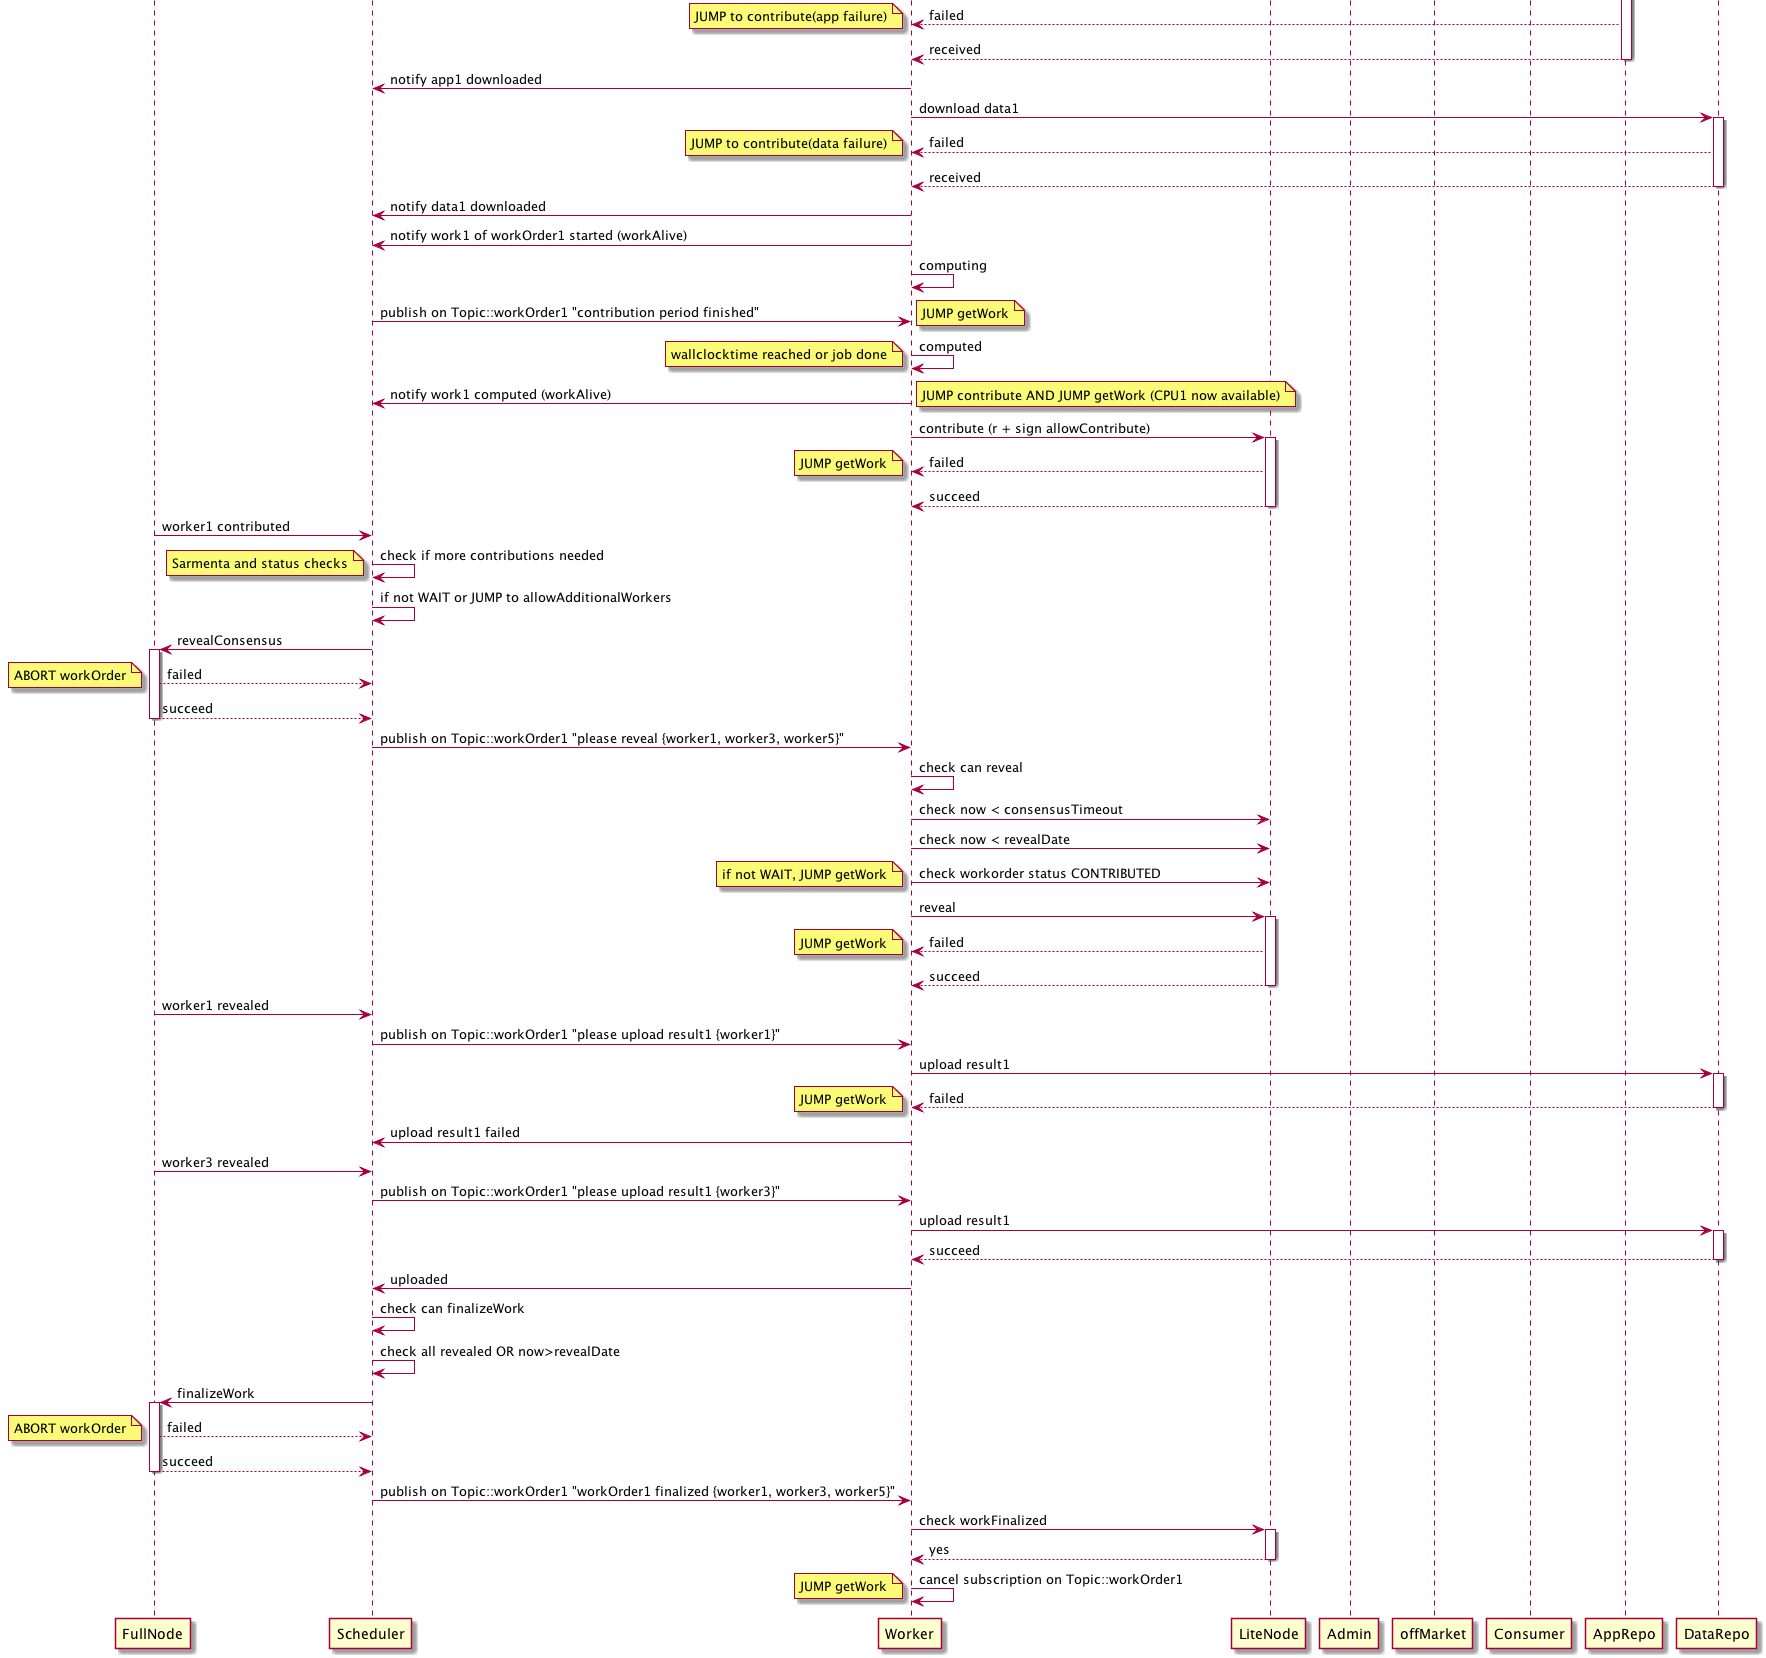
\includegraphics[width=1.3\linewidth]{4-Requirements/figs/iexec-core-sequence-diagram-part-2.png}
            }
            \caption{iExec core sequence diagram - part 2}
        \end{figure}

%******************************** Section 3.3 *********************************%
\section{Requirements}
    \subsection{Functional Requirements}
        The project aims to povide a certain number of functionalities, some of them are absolutely mondatory
        and some others depend on the use case. The main features are listed below.
        \begin{itemize}
            \item \textbf{Execute jobs sent by the middleware:} The worker is a part of iExec's infrastructure, so it
            should execute any type of job sent by XtremWeb middleware, the source of these tasks is blockchain
            dapps that need computation resources. The only constraint that those tasks should repect is the
            specs limitation of the device, Raspberry Pi cards for instance. It's the responsibility of
            the dapps developer and the task sender to deal with this contraint.

            \item \textbf{Ability to prove execution:} The proof-of-contribution\cite{POCO} is the protocole that
            verifies the execution of tasks, so the worker should be able to contribute to the process of the
            verification. In order to achieve that, the worker should have an identity represented by its
            blockchain wallet and its account in the iExec ecosystem.

            \item \textbf{Accomplish the mission of an IoT device:} The worker is always available to execute tasks sent by
            users, but it can also be considered as an IoT device that processes/sends data collected by its sensors.
            For instance, the worker can be a surveillance camera and analyse the video stream to detect motions or
            a weather station that collects informations about the temprature, the humidity, the wind speed ...etc.

            \item \textbf{Ability to manage a cluster of workers:} The project is meant to be applicable on a large number of
            workers, so it is hard to manage them seperatly, that is why it is necessary to have a way to manage them
            easily as a cluster.
        \end{itemize}

    \subsection{Non-Functional Requirements}
        The project emphasizes some extremely important non-functional requirements. Those key specifications should be
        respected in order to maintain the spirit of the project.
        \begin{itemize}
            \item \textbf{Positive energy:} One of the main features of this project is to eliminate the energy cost and
            design a system that is totally green and nature friendly. The worker is powered by solar energy and would
            produce more energy than it consumes. The electricity is saved in a battery to avoid climate's change effects.
            The objectif is to charge the battery with enough electricity for two days.

            \item \textbf{Support ARM architecture:} Who says IoT says ARM\cite{ARM} because this architecture is the
            omnipresent architecture in the IoT ecosystem, so the project has absolutely to support it. The challenge
            would be to build binaries for ARM using non-ARM hardware.
        \end{itemize}

%******************************** Section 3.4 *********************************%
\section{Conclusion}
    After understanding the global architecture of the iExec environment and defining the roles of the different components,
    we identified the functional and non-functional requirements of the project. Those requirements would lead us to the next
    part where we design our system and detail its technical specifications.